\documentclass[11pt,a4paper]{article}
\usepackage[margin=22mm]{geometry}
\usepackage[utf8]{inputenc}
\usepackage[T1]{fontenc}
\usepackage{lmodern}
\usepackage{amsmath,amssymb,bm}
\usepackage{graphicx}
\usepackage{booktabs}
\usepackage{longtable}
\usepackage{caption}
\usepackage{natbib}
\usepackage{adjustbox}
\usepackage{listings}
\usepackage{xcolor}
\usepackage[hidelinks]{hyperref}
\usepackage{microtype}
\graphicspath{{figures/}}
\captionsetup{font=small,labelfont=bf,justification=justified}
\renewcommand{\thetable}{S\arabic{table}}
\setlength{\LTcapwidth}{\textwidth}
\captionsetup[longtable]{justification=justified,singlelinecheck=false}
\renewcommand{\thefigure}{S\arabic{figure}}
\renewcommand{\theequation}{S\arabic{equation}}
\renewcommand{\thesection}{S\arabic{section}}
\lstset{basicstyle=\ttfamily\footnotesize,breaklines=true,frame=single,columns=fullflexible,backgroundcolor=\color{gray!5}}
\DeclareMathOperator*{\argmax}{arg\,max}
\DeclareMathOperator{\median}{median}
\newcommand{\bS}{\mathbf{S}}

\title{Supplementary information\\[4pt]\large Clustering trajectories of modelled estimates: an uncertainty aware framework, with an application to global cardiovascular disease burden, 1990 to 2023}
\author{Eben Afrifa-Yamoah\\ \small School of Science, Edith Cowan University, Perth, Western Australia}
\date{3 October 2026}

\begin{document}
\maketitle

\noindent This document contains the country-level results, the sensitivity tables referred to in the main text, a worked description of the data extraction, and the reproduction instructions. Section and table numbers are prefixed S. Colour conventions follow the main text: orange is the stalled cluster, blue the sustained-decline cluster, green the third cluster found only in the narrow-interval analysis, and dark grey the unassigned class.

\tableofcontents

\section{Data extraction}

\subsection{Connector calls}

All series were retrieved through the IHME GBD 2023 Model Context Protocol connector with the \texttt{get\_multi\_location\_trend} tool. The connector caps a single response by token budget rather than by row count, so the number of rows returned depends on the output format and the measure: about 667 location-years for DALYs in JSON format, about 476 for deaths in JSON format (the deaths output carries more columns), and about 714 for deaths in CSV format. Each global series was therefore assembled from twelve calls, partitioned by World Bank income group and year window as in Table~\ref{tab:calls}. The four income groups partition the 203 countries that carry a World Bank code; Hong Kong and Macao appear under their own codes but sit under China in the GBD hierarchy and were dropped, and Tuvalu carries no code in the connector.

\begin{table}[h]
\centering\small
\caption{Extraction schedule. Each cell is one connector call; windows were sized so that every call stays below the response cap.}
\label{tab:calls}
\begin{tabular}{lrl}
\toprule
World Bank income group & Countries & Year windows \\
\midrule
Low income & 26 & 1990 to 2006; 2007 to 2023 \\
Lower middle income & 51 & 1990 to 2001; 2002 to 2013; 2014 to 2023 \\
Upper middle income & 54 & 1990 to 2001; 2002 to 2013; 2014 to 2023 \\
High income & 72 & 1990 to 1998; 1999 to 2007; 2008 to 2016; 2017 to 2023 \\
\bottomrule
\end{tabular}
\end{table}

Two fields were retained per country-year: the age-standardised rate for both sexes, and the all-ages rate with its 95\% uncertainty interval. The connector does not return an interval for the age-standardised rate, and does not expose the posterior draws from which the published intervals are computed. The Socio-demographic Index for 2023 was retrieved for all 204 locations in one call, and the GBD super region of each country was taken from the location hierarchy returned by the ranking tool.

\subsection{Interval width as a measurement quality proxy}

The quantity $w_i$ of main-text equation (2) is the country mean of the per-observation log-scale standard deviation implied by the published interval of the all-ages DALY rate. Figure 7a of the main text shows its distribution by super region. The median is 0.024 in Central and Eastern Europe and Central Asia, 0.033 in Latin America and the Caribbean, 0.038 in the high-income super region, 0.067 in North Africa and the Middle East, 0.069 in Southeast Asia, East Asia and Oceania, 0.097 in South Asia and 0.107 in sub-Saharan Africa. The proxy reflects every source of modelling uncertainty, not only the sparseness of primary data, and would be replaced by GBD's published vital registration star ratings in a final analysis.


\section{Country-level results}

Table~\ref{S1} lists every country in the analysis set with its super region, World Bank income group, 2023 SDI, percentage change in the age-standardised DALY and death rates from 1990 to 2023, year of the cardiovascular DALY peak, interval width, and the assigned cluster and membership probability under the primary analysis, the deaths analysis and the 2000 to 2023 window. Cluster 1 is stalled, cluster 2 sustained decline, and 0 unassigned (membership probability below 0.70).

\begingroup\scriptsize\setlength{\tabcolsep}{3.2pt}
\begin{longtable}{llrrrrrrrrrrrr}
\caption{Country level results. Region codes: CEECA, Central Europe, Eastern Europe and Central Asia; HI, high income; LAC, Latin America and Caribbean; NAME, North Africa and Middle East; SA, South Asia; SEAO, Southeast Asia, East Asia and Oceania; SSA, sub-Saharan Africa. Inc.: World Bank income group (L low, LM lower middle, UM upper middle, H high). $\Delta$DALY and $\Delta$deaths: percentage change in the age-standardised rate, 1990 to 2023. Peak: year of maximum centred DALY trajectory. $w_i$: mean log-scale standard deviation of the published interval. $a_i$: assigned cluster (1 stalled, 2 sustained decline, 0 unassigned) and $p_i$: membership probability, for the primary DALY analysis; superscript d, the deaths analysis; superscript w, the 2000 to 2023 window.}\label{S1}\\
\toprule
Country & Region & Inc. & SDI & $\Delta$DALY & $\Delta$deaths & Peak & $w_i$ & $a_i$ & $p_i$ & $a_i^{\mathrm{d}}$ & $p_i^{\mathrm{d}}$ & $a_i^{\mathrm{w}}$ & $p_i^{\mathrm{w}}$ \\
\midrule
\endfirsthead
\multicolumn{14}{l}{\small\textit{Table \thetable{} continued}}\\
\toprule
Country & Region & Inc. & SDI & $\Delta$DALY & $\Delta$deaths & Peak & $w_i$ & $a_i$ & $p_i$ & $a_i^{\mathrm{d}}$ & $p_i^{\mathrm{d}}$ & $a_i^{\mathrm{w}}$ & $p_i^{\mathrm{w}}$ \\
\midrule
\endhead
\bottomrule
\endfoot
Albania & CEECA & UM & 0.7068 & -41.5 & -37.8 & 1990 & 0.043 & 0 & 0.65 & 0 & 0.34 & 2 & 0.85 \\
Armenia & CEECA & UM & 0.7173 & -51.6 & -50.5 & 1993 & 0.027 & 2 & 0.99 & 2 & 0.92 & 2 & 1.00 \\
Azerbaijan & CEECA & UM & 0.7053 & -32.5 & -29.1 & 1994 & 0.041 & 0 & 0.60 & 1 & 0.89 & 2 & 0.83 \\
Belarus & CEECA & UM & 0.8036 & -23.1 & -21.6 & 1998 & 0.018 & 0 & 0.69 & 0 & 0.29 & 2 & 0.99 \\
Bosnia and Herzegovina & CEECA & UM & 0.7129 & -40.7 & -37.9 & 1990 & 0.033 & 0 & 0.64 & 0 & 0.33 & 2 & 0.79 \\
Bulgaria & CEECA & H & 0.7708 & -34.8 & -34.3 & 1997 & 0.018 & 0 & 0.66 & 0 & 0.35 & 2 & 0.84 \\
Croatia & CEECA & H & 0.7821 & -56.2 & -54.6 & 1990 & 0.021 & 2 & 1.00 & 2 & 0.95 & 2 & 1.00 \\
Czechia & CEECA & H & 0.8310 & -64.7 & -63.1 & 1990 & 0.024 & 2 & 1.00 & 2 & 1.00 & 2 & 1.00 \\
Estonia & CEECA & H & 0.8549 & -64.3 & -62.4 & 1994 & 0.023 & 2 & 1.00 & 2 & 1.00 & 2 & 1.00 \\
Georgia & CEECA & UM & 0.7546 & -48.4 & -48.9 & 1991 & 0.026 & 2 & 0.94 & 2 & 0.79 & 2 & 1.00 \\
Hungary & CEECA & H & 0.7935 & -49.8 & -45.7 & 1991 & 0.019 & 2 & 1.00 & 2 & 0.91 & 2 & 0.88 \\
Kazakhstan & CEECA & UM & 0.7272 & -42.8 & -44.8 & 2006 & 0.021 & 2 & 0.92 & 2 & 0.90 & 2 & 1.00 \\
Kyrgyzstan & CEECA & LM & 0.6252 & -32.9 & -24.6 & 1995 & 0.023 & 2 & 0.82 & 0 & 0.17 & 2 & 1.00 \\
Latvia & CEECA & H & 0.8508 & -42.5 & -43.3 & 1994 & 0.020 & 2 & 0.96 & 2 & 0.88 & 2 & 1.00 \\
Lithuania & CEECA & H & 0.8562 & -43.3 & -42.0 & 1994 & 0.021 & 2 & 0.89 & 0 & 0.62 & 2 & 1.00 \\
Mongolia & CEECA & UM & 0.6597 & -44.2 & -43.9 & 1997 & 0.047 & 2 & 0.92 & 2 & 0.90 & 2 & 1.00 \\
Montenegro & CEECA & UM & 0.7886 & -36.0 & -35.1 & 1997 & 0.036 & 2 & 0.71 & 0 & 0.40 & 2 & 0.99 \\
North Macedonia & CEECA & UM & 0.7585 & -42.2 & -37.8 & 1995 & 0.026 & 2 & 0.82 & 0 & 0.43 & 2 & 1.00 \\
Poland & CEECA & H & 0.8470 & -62.5 & -60.8 & 1991 & 0.024 & 2 & 1.00 & 2 & 1.00 & 2 & 1.00 \\
Republic of Moldova & CEECA & UM & 0.7337 & -41.3 & -46.7 & 1995 & 0.020 & 2 & 0.91 & 2 & 0.91 & 2 & 1.00 \\
Romania & CEECA & H & 0.7687 & -43.0 & -42.5 & 1996 & 0.017 & 2 & 0.99 & 2 & 0.87 & 2 & 0.99 \\
Russian Federation & CEECA & H & 0.8225 & -30.5 & -36.4 & 2003 & 0.015 & 2 & 0.90 & 2 & 0.89 & 2 & 1.00 \\
Serbia & CEECA & UM & 0.7845 & -46.7 & -42.1 & 1996 & 0.030 & 2 & 0.99 & 2 & 0.87 & 2 & 1.00 \\
Slovakia & CEECA & H & 0.8131 & -55.7 & -52.7 & 1990 & 0.029 & 2 & 1.00 & 2 & 0.94 & 2 & 1.00 \\
Slovenia & CEECA & H & 0.8449 & -67.7 & -66.7 & 1990 & 0.028 & 2 & 1.00 & 2 & 1.00 & 2 & 1.00 \\
Tajikistan & CEECA & LM & 0.5512 &  -2.7 &   4.5 & 1994 & 0.052 & 1 & 0.93 & 1 & 1.00 & 1 & 0.96 \\
Turkmenistan & CEECA & UM & 0.6822 & -14.0 & -13.4 & 1996 & 0.024 & 0 & 0.43 & 1 & 0.83 & 2 & 0.80 \\
Ukraine & CEECA & UM & 0.7645 & -30.1 & -32.2 & 1995 & 0.019 & 2 & 0.71 & 0 & 0.32 & 2 & 1.00 \\
Uzbekistan & CEECA & LM & 0.6321 & -18.0 & -15.3 & 1995 & 0.021 & 1 & 0.88 & 1 & 0.93 & 0 & 0.43 \\
Andorra & HI & H & 0.8799 & -43.6 & -46.8 & 1990 & 0.080 & 2 & 0.89 & 2 & 0.92 & 2 & 0.76 \\
Argentina & HI & UM & 0.7647 & -52.2 & -53.3 & 1990 & 0.025 & 2 & 1.00 & 2 & 0.95 & 2 & 0.82 \\
Australia & HI & H & 0.8529 & -67.2 & -71.0 & 1990 & 0.039 & 2 & 1.00 & 2 & 1.00 & 2 & 1.00 \\
Austria & HI & H & 0.8540 & -57.5 & -57.6 & 1990 & 0.036 & 2 & 1.00 & 2 & 1.00 & 2 & 0.99 \\
Belgium & HI & H & 0.8770 & -62.5 & -63.7 & 1990 & 0.039 & 2 & 1.00 & 2 & 1.00 & 2 & 1.00 \\
Brunei Darussalam & HI & H & 0.8324 & -45.7 & -48.1 & 1991 & 0.054 & 2 & 0.96 & 2 & 0.94 & 2 & 0.87 \\
Canada & HI & H & 0.8873 & -52.2 & -57.1 & 1990 & 0.037 & 2 & 1.00 & 2 & 1.00 & 2 & 0.88 \\
Chile & HI & H & 0.7885 & -55.5 & -59.4 & 1990 & 0.026 & 2 & 1.00 & 2 & 0.98 & 2 & 0.98 \\
Cyprus & HI & H & 0.8558 & -61.4 & -59.7 & 1990 & 0.061 & 2 & 1.00 & 2 & 1.00 & 2 & 1.00 \\
Denmark & HI & H & 0.9160 & -69.0 & -69.8 & 1990 & 0.034 & 2 & 1.00 & 2 & 1.00 & 2 & 1.00 \\
Finland & HI & H & 0.8908 & -59.2 & -55.2 & 1990 & 0.034 & 2 & 1.00 & 2 & 0.98 & 2 & 1.00 \\
France & HI & H & 0.8611 & -48.9 & -56.2 & 1990 & 0.048 & 2 & 1.00 & 2 & 1.00 & 2 & 0.97 \\
Germany & HI & H & 0.8786 & -55.9 & -56.6 & 1990 & 0.039 & 2 & 1.00 & 2 & 1.00 & 2 & 0.95 \\
Greece & HI & H & 0.8312 & -51.7 & -55.4 & 1990 & 0.031 & 2 & 1.00 & 2 & 1.00 & 2 & 1.00 \\
Greenland & HI & H & 0.8602 & -59.4 & -57.4 & 1990 & 0.057 & 2 & 1.00 & 2 & 1.00 & 2 & 1.00 \\
Iceland & HI & H & 0.8890 & -57.4 & -55.6 & 1990 & 0.039 & 2 & 1.00 & 2 & 1.00 & 2 & 1.00 \\
Ireland & HI & H & 0.9069 & -70.4 & -68.9 & 1990 & 0.031 & 2 & 1.00 & 2 & 1.00 & 2 & 1.00 \\
Israel & HI & H & 0.8409 & -70.2 & -71.5 & 1992 & 0.038 & 2 & 1.00 & 2 & 1.00 & 2 & 1.00 \\
Italy & HI & H & 0.8344 & -56.9 & -57.8 & 1990 & 0.049 & 2 & 1.00 & 2 & 1.00 & 2 & 0.98 \\
Japan & HI & H & 0.8759 & -50.7 & -59.3 & 1990 & 0.048 & 2 & 1.00 & 2 & 1.00 & 2 & 0.84 \\
Luxembourg & HI & H & 0.8948 & -68.5 & -68.2 & 1990 & 0.033 & 2 & 1.00 & 2 & 1.00 & 2 & 1.00 \\
Malta & HI & H & 0.8305 & -65.9 & -65.9 & 1990 & 0.034 & 2 & 1.00 & 2 & 1.00 & 2 & 1.00 \\
Monaco & HI & H & 0.9227 & -75.5 & -76.5 & 1990 & 0.127 & 2 & 1.00 & 2 & 1.00 & 2 & 1.00 \\
Netherlands & HI & H & 0.9084 & -63.4 & -62.5 & 1990 & 0.036 & 2 & 1.00 & 2 & 1.00 & 2 & 1.00 \\
New Zealand & HI & H & 0.8664 & -59.6 & -58.2 & 1990 & 0.036 & 2 & 1.00 & 2 & 1.00 & 2 & 0.99 \\
Norway & HI & H & 0.9169 & -68.1 & -68.9 & 1990 & 0.042 & 2 & 1.00 & 2 & 1.00 & 2 & 1.00 \\
Portugal & HI & H & 0.7865 & -68.4 & -71.1 & 1990 & 0.035 & 2 & 1.00 & 2 & 1.00 & 2 & 1.00 \\
Republic of Korea & HI & H & 0.8917 & -77.6 & -78.6 & 1990 & 0.049 & 2 & 1.00 & 2 & 1.00 & 2 & 1.00 \\
San Marino & HI & H & 0.8830 & -60.9 & -65.6 & 1990 & 0.067 & 2 & 1.00 & 2 & 1.00 & 2 & 1.00 \\
Singapore & HI & H & 0.8700 & -67.3 & -69.6 & 1990 & 0.029 & 2 & 1.00 & 2 & 1.00 & 2 & 1.00 \\
Spain & HI & H & 0.8118 & -57.2 & -61.8 & 1990 & 0.041 & 2 & 1.00 & 2 & 1.00 & 2 & 0.99 \\
Sweden & HI & H & 0.9109 & -59.7 & -61.7 & 1990 & 0.039 & 2 & 1.00 & 2 & 1.00 & 2 & 1.00 \\
Switzerland & HI & H & 0.9461 & -63.7 & -62.1 & 1990 & 0.042 & 2 & 1.00 & 2 & 1.00 & 2 & 1.00 \\
United Kingdom & HI & H & 0.8804 & -59.9 & -62.2 & 1990 & 0.032 & 2 & 1.00 & 2 & 1.00 & 2 & 1.00 \\
United States of America & HI & H & 0.8765 & -40.5 & -45.8 & 1990 & 0.036 & 2 & 0.85 & 2 & 0.92 & 2 & 0.76 \\
Uruguay & HI & H & 0.7454 & -50.7 & -52.9 & 1990 & 0.027 & 2 & 1.00 & 2 & 0.97 & 2 & 0.94 \\
Antigua and Barbuda & LAC & H & 0.7559 & -45.3 & -47.0 & 1990 & 0.032 & 2 & 0.92 & 2 & 0.93 & 2 & 0.75 \\
Bahamas & LAC & H & 0.8136 & -22.0 & -18.2 & 1990 & 0.027 & 1 & 0.99 & 1 & 1.00 & 1 & 0.98 \\
Barbados & LAC & H & 0.7548 & -37.3 & -39.7 & 1990 & 0.031 & 2 & 0.76 & 2 & 0.82 & 1 & 0.78 \\
Belize & LAC & UM & 0.6285 & -32.2 & -32.1 & 2000 & 0.034 & 0 & 0.64 & 0 & 0.35 & 2 & 0.83 \\
Bermuda & LAC & H & 0.8269 & -55.1 & -56.9 & 1990 & 0.033 & 2 & 1.00 & 2 & 1.00 & 2 & 0.84 \\
Bolivia & LAC & LM & 0.6317 & -36.1 & -39.7 & 1991 & 0.112 & 0 & 0.34 & 0 & 0.33 & 0 & 0.64 \\
Brazil & LAC & UM & 0.6839 & -52.0 & -54.8 & 1990 & 0.024 & 2 & 1.00 & 2 & 0.97 & 2 & 0.98 \\
Colombia & LAC & UM & 0.6888 & -52.9 & -52.8 & 1990 & 0.024 & 2 & 1.00 & 2 & 0.95 & 2 & 0.84 \\
Costa Rica & LAC & UM & 0.7154 & -36.6 & -37.2 & 1993 & 0.027 & 2 & 0.88 & 2 & 0.91 & 2 & 0.78 \\
Cuba & LAC & UM & 0.6949 & -36.2 & -36.8 & 1990 & 0.024 & 0 & 0.38 & 0 & 0.35 & 1 & 0.90 \\
Dominica & LAC & UM & 0.7537 & -22.5 & -23.4 & 1992 & 0.046 & 1 & 0.99 & 1 & 0.96 & 1 & 1.00 \\
Dominican Republic & LAC & UM & 0.6581 &  -4.6 &   5.4 & 1990 & 0.042 & 1 & 1.00 & 1 & 1.00 & 1 & 1.00 \\
Ecuador & LAC & UM & 0.6910 & -36.1 & -34.1 & 1994 & 0.022 & 2 & 0.94 & 2 & 0.93 & 2 & 0.80 \\
El Salvador & LAC & UM & 0.6082 & -28.3 & -18.5 & 1990 & 0.046 & 0 & 0.18 & 1 & 1.00 & 1 & 1.00 \\
Grenada & LAC & UM & 0.6781 & -42.2 & -45.3 & 1991 & 0.034 & 2 & 0.83 & 2 & 0.93 & 0 & 0.56 \\
Guatemala & LAC & UM & 0.5538 & -31.9 & -21.3 & 1993 & 0.028 & 0 & 0.20 & 1 & 1.00 & 1 & 1.00 \\
Guyana & LAC & H & 0.6957 & -43.2 & -43.3 & 1990 & 0.030 & 2 & 0.72 & 0 & 0.41 & 0 & 0.47 \\
Haiti & LAC & LM & 0.4638 &   1.4 &   6.4 & 2023 & 0.100 & 1 & 1.00 & 1 & 1.00 & 1 & 1.00 \\
Honduras & LAC & LM & 0.5203 & -10.4 &   4.2 & 1998 & 0.076 & 1 & 1.00 & 1 & 1.00 & 1 & 0.98 \\
Jamaica & LAC & UM & 0.6919 & -21.5 & -26.2 & 1990 & 0.034 & 1 & 1.00 & 1 & 1.00 & 1 & 1.00 \\
Mexico & LAC & UM & 0.6934 & -17.5 & -17.0 & 1994 & 0.025 & 1 & 1.00 & 1 & 1.00 & 1 & 1.00 \\
Nicaragua & LAC & LM & 0.5357 & -23.3 & -13.8 & 1990 & 0.042 & 1 & 1.00 & 1 & 1.00 & 1 & 1.00 \\
Panama & LAC & H & 0.7154 & -31.4 & -32.2 & 1990 & 0.030 & 0 & 0.35 & 0 & 0.36 & 1 & 0.99 \\
Paraguay & LAC & UM & 0.6741 & -21.5 & -18.6 & 1990 & 0.039 & 1 & 0.99 & 1 & 1.00 & 1 & 1.00 \\
Peru & LAC & UM & 0.6856 & -36.8 & -38.8 & 1994 & 0.051 & 2 & 0.92 & 2 & 0.94 & 0 & 0.65 \\
Puerto Rico & LAC & H & 0.8475 & -53.3 & -55.9 & 1990 & 0.031 & 2 & 1.00 & 2 & 1.00 & 2 & 1.00 \\
Saint Kitts and Nevis & LAC & H & 0.7545 & -52.8 & -51.8 & 1990 & 0.027 & 2 & 1.00 & 2 & 0.96 & 2 & 0.86 \\
Saint Lucia & LAC & UM & 0.7029 & -51.5 & -53.6 & 1990 & 0.035 & 2 & 1.00 & 2 & 0.96 & 2 & 0.80 \\
Saint Vincent and the Grenadines & LAC & UM & 0.6585 & -27.8 & -31.3 & 1994 & 0.034 & 0 & 0.40 & 0 & 0.34 & 1 & 0.88 \\
Suriname & LAC & UM & 0.6549 & -30.1 & -30.9 & 1992 & 0.036 & 0 & 0.40 & 0 & 0.27 & 0 & 0.69 \\
Trinidad and Tobago & LAC & H & 0.7705 & -42.9 & -42.1 & 1990 & 0.023 & 2 & 0.94 & 2 & 0.93 & 2 & 0.79 \\
United States Virgin Islands & LAC & H & 0.8302 & -52.6 & -62.7 & 1990 & 0.034 & 2 & 1.00 & 2 & 1.00 & 2 & 0.94 \\
Venezuela & LAC & UM & 0.5802 & -12.6 &  -9.7 & 1990 & 0.022 & 0 & 0.18 & 1 & 1.00 & 1 & 1.00 \\
Afghanistan & NAME & L & 0.3337 & -29.0 & -25.4 & 1990 & 0.070 & 0 & 0.27 & 1 & 0.88 & 1 & 0.72 \\
Algeria & NAME & UM & 0.6578 & -39.2 & -39.3 & 1990 & 0.081 & 0 & 0.57 & 0 & 0.35 & 0 & 0.44 \\
Bahrain & NAME & H & 0.7843 & -65.7 & -65.8 & 1990 & 0.050 & 2 & 1.00 & 2 & 1.00 & 2 & 1.00 \\
Egypt & NAME & LM & 0.6765 &  -6.7 &   6.2 & 2003 & 0.060 & 1 & 1.00 & 1 & 1.00 & 1 & 0.97 \\
Iran & NAME & UM & 0.7176 & -60.6 & -59.0 & 1990 & 0.065 & 2 & 1.00 & 2 & 0.98 & 2 & 0.99 \\
Iraq & NAME & UM & 0.6539 & -23.9 & -21.1 & 1998 & 0.068 & 0 & 0.44 & 0 & 0.20 & 2 & 0.74 \\
Jordan & NAME & LM & 0.7204 & -50.6 & -46.8 & 1992 & 0.052 & 2 & 0.99 & 2 & 0.89 & 2 & 1.00 \\
Kuwait & NAME & H & 0.8771 & -54.2 & -54.7 & 1990 & 0.026 & 2 & 1.00 & 2 & 0.98 & 2 & 1.00 \\
Lebanon & NAME & LM & 0.7237 & -21.1 & -19.8 & 2020 & 0.091 & 1 & 0.98 & 1 & 1.00 & 1 & 1.00 \\
Libya & NAME & UM & 0.7705 & -23.8 & -15.2 & 1990 & 0.077 & 1 & 0.93 & 1 & 1.00 & 1 & 0.90 \\
Morocco & NAME & LM & 0.6124 & -33.9 & -30.6 & 1990 & 0.063 & 0 & 0.53 & 0 & 0.29 & 0 & 0.63 \\
Oman & NAME & H & 0.7812 & -54.1 & -47.7 & 1990 & 0.067 & 2 & 0.80 & 0 & 0.31 & 2 & 0.85 \\
Palestine & NAME & LM & 0.6380 & -46.7 & -43.4 & 1990 & 0.044 & 2 & 0.95 & 2 & 0.71 & 2 & 1.00 \\
Qatar & NAME & H & 0.8596 & -64.5 & -64.6 & 1992 & 0.069 & 2 & 1.00 & 2 & 1.00 & 2 & 1.00 \\
Saudi Arabia & NAME & H & 0.8284 & -33.6 & -29.6 & 1990 & 0.064 & 1 & 0.99 & 1 & 1.00 & 1 & 1.00 \\
Sudan & NAME & L & 0.5731 & -43.5 & -38.4 & 1990 & 0.084 & 2 & 0.78 & 0 & 0.38 & 2 & 0.81 \\
Syrian Arab Republic & NAME & L & 0.5887 & -43.2 & -29.8 & 1992 & 0.043 & 2 & 0.96 & 0 & 0.34 & 2 & 0.97 \\
Tunisia & NAME & LM & 0.6837 & -39.9 & -46.1 & 1990 & 0.088 & 2 & 0.77 & 2 & 0.87 & 2 & 0.83 \\
Türkiye & NAME & UM & 0.7310 & -54.7 & -50.4 & 1990 & 0.057 & 2 & 1.00 & 2 & 0.93 & 2 & 0.88 \\
United Arab Emirates & NAME & H & 0.8622 & -51.5 & -39.1 & 1990 & 0.180 & 2 & 0.91 & 0 & 0.18 & 2 & 0.79 \\
Yemen & NAME & L & 0.4464 & -42.9 & -39.0 & 1990 & 0.071 & 2 & 0.77 & 0 & 0.38 & 2 & 0.78 \\
Bangladesh & SA & LM & 0.5171 &  22.0 &  37.2 & 2012 & 0.067 & 1 & 1.00 & 1 & 1.00 & 1 & 1.00 \\
Bhutan & SA & LM & 0.5243 & -21.5 & -27.5 & 1997 & 0.119 & 0 & 0.38 & 0 & 0.28 & 0 & 0.63 \\
India & SA & LM & 0.6070 & -19.6 & -12.1 & 1990 & 0.062 & 1 & 1.00 & 1 & 1.00 & 1 & 1.00 \\
Nepal & SA & LM & 0.4710 & -21.0 & -21.3 & 1999 & 0.097 & 0 & 0.38 & 0 & 0.24 & 0 & 0.61 \\
Pakistan & SA & LM & 0.5127 &  -2.1 &  -2.6 & 2005 & 0.113 & 1 & 1.00 & 1 & 1.00 & 1 & 0.99 \\
American Samoa & SEAO & H & 0.7430 &  -9.4 & -13.0 & 1999 & 0.068 & 1 & 0.99 & 1 & 0.98 & 1 & 0.96 \\
Cambodia & SEAO & LM & 0.5000 & -26.0 & -18.7 & 1990 & 0.115 & 0 & 0.25 & 1 & 0.95 & 1 & 0.79 \\
China & SEAO & UM & 0.7275 & -59.7 & -58.1 & 1990 & 0.048 & 2 & 1.00 & 2 & 1.00 & 2 & 1.00 \\
Korea, DPR & SEAO & L & 0.5771 &  -5.7 &  -7.6 & 2004 & 0.074 & 1 & 1.00 & 1 & 1.00 & 1 & 0.96 \\
Fiji & SEAO & UM & 0.6864 &  -4.2 &  -0.3 & 1998 & 0.049 & 1 & 1.00 & 1 & 1.00 & 1 & 0.98 \\
Guam & SEAO & H & 0.8119 &   0.0 & -15.1 & 1999 & 0.027 & 1 & 1.00 & 1 & 1.00 & 1 & 1.00 \\
Indonesia & SEAO & UM & 0.6657 &  -8.5 & -15.1 & 2013 & 0.069 & 1 & 1.00 & 1 & 1.00 & 1 & 1.00 \\
Kiribati & SEAO & LM & 0.5427 &  -4.5 &  -5.7 & 1998 & 0.080 & 1 & 1.00 & 1 & 1.00 & 1 & 0.99 \\
Lao People's Democratic Republic & SEAO & LM & 0.5150 &  -2.4 &  -4.6 & 1994 & 0.110 & 1 & 1.00 & 1 & 1.00 & 1 & 0.98 \\
Malaysia & SEAO & UM & 0.7704 & -35.8 & -41.1 & 1990 & 0.046 & 0 & 0.63 & 2 & 0.80 & 2 & 0.72 \\
Maldives & SEAO & UM & 0.6610 & -43.4 & -26.5 & 1991 & 0.060 & 2 & 0.97 & 0 & 0.36 & 2 & 0.87 \\
Marshall Islands & SEAO & UM & 0.6055 &   3.3 &   4.5 & 2021 & 0.102 & 1 & 1.00 & 1 & 1.00 & 1 & 1.00 \\
Mauritius & SEAO & UM & 0.7363 & -38.1 & -37.7 & 1990 & 0.022 & 2 & 0.90 & 2 & 0.93 & 2 & 0.74 \\
Micronesia & SEAO & LM & 0.5968 & -32.8 & -32.5 & 1990 & 0.078 & 0 & 0.41 & 0 & 0.26 & 0 & 0.51 \\
Myanmar & SEAO & LM & 0.5320 & -17.0 & -17.5 & 2008 & 0.106 & 1 & 0.93 & 1 & 0.98 & 1 & 0.88 \\
Nauru & SEAO & H & 0.6264 &   4.8 &   3.6 & 2005 & 0.122 & 1 & 1.00 & 1 & 1.00 & 1 & 0.93 \\
Northern Mariana Islands & SEAO & H & 0.7911 & -12.4 & -13.1 & 1999 & 0.068 & 1 & 1.00 & 1 & 1.00 & 1 & 0.99 \\
Palau & SEAO & H & 0.7559 & -20.6 & -21.0 & 1990 & 0.068 & 1 & 0.88 & 1 & 0.92 & 1 & 0.80 \\
Papua New Guinea & SEAO & LM & 0.4290 &  -6.6 &  -8.7 & 2011 & 0.103 & 1 & 0.99 & 1 & 1.00 & 1 & 0.99 \\
Philippines & SEAO & LM & 0.6694 &  -5.2 & -10.3 & 2021 & 0.039 & 1 & 1.00 & 1 & 1.00 & 1 & 1.00 \\
Samoa & SEAO & LM & 0.6045 &   7.6 &  10.0 & 2023 & 0.081 & 1 & 1.00 & 1 & 1.00 & 1 & 1.00 \\
Seychelles & SEAO & H & 0.7530 & -43.0 & -43.0 & 1991 & 0.049 & 2 & 0.87 & 2 & 0.73 & 2 & 0.98 \\
Solomon Islands & SEAO & LM & 0.4580 &  15.7 &  10.7 & 2023 & 0.088 & 1 & 1.00 & 1 & 1.00 & 1 & 1.00 \\
Sri Lanka & SEAO & LM & 0.7307 & -31.7 & -30.9 & 1990 & 0.040 & 0 & 0.69 & 0 & 0.34 & 2 & 0.89 \\
Taiwan & SEAO & H & 0.8815 & -58.4 & -64.2 & 1990 & 0.029 & 2 & 1.00 & 2 & 1.00 & 2 & 0.84 \\
Thailand & SEAO & UM & 0.6872 & -42.2 & -54.2 & 1995 & 0.060 & 2 & 0.98 & 2 & 1.00 & 2 & 1.00 \\
Timor-Leste & SEAO & LM & 0.4846 & -16.7 & -23.1 & 1990 & 0.108 & 1 & 0.97 & 1 & 0.96 & 1 & 1.00 \\
Tonga & SEAO & UM & 0.6360 &   3.0 &   3.3 & 2009 & 0.076 & 1 & 1.00 & 1 & 1.00 & 1 & 1.00 \\
Tuvalu & SEAO & UM & 0.6112 &   0.3 &  -4.2 & 2021 & 0.082 & 1 & 1.00 & 1 & 1.00 & 1 & 1.00 \\
Vanuatu & SEAO & LM & 0.4765 &  -1.2 &  -2.8 & 1994 & 0.086 & 1 & 1.00 & 1 & 1.00 & 1 & 1.00 \\
Viet Nam & SEAO & LM & 0.6430 & -31.4 & -35.5 & 1990 & 0.064 & 0 & 0.25 & 0 & 0.26 & 1 & 0.82 \\
Angola & SSA & LM & 0.4991 & -16.7 & -17.2 & 1990 & 0.121 & 1 & 0.98 & 1 & 0.98 & 1 & 0.96 \\
Benin & SSA & LM & 0.4064 & -31.2 & -30.9 & 1990 & 0.104 & 1 & 0.86 & 0 & 0.09 & 1 & 0.96 \\
Botswana & SSA & UM & 0.6776 & -26.3 & -25.8 & 2001 & 0.099 & 0 & 0.52 & 0 & 0.32 & 2 & 0.82 \\
Burkina Faso & SSA & L & 0.3067 & -16.3 & -17.5 & 1990 & 0.096 & 1 & 0.94 & 1 & 0.97 & 1 & 0.92 \\
Burundi & SSA & L & 0.3072 &   7.4 &  12.3 & 2021 & 0.141 & 1 & 1.00 & 1 & 1.00 & 1 & 1.00 \\
Cabo Verde & SSA & LM & 0.5624 & -12.7 & -16.0 & 1995 & 0.073 & 1 & 0.98 & 1 & 0.91 & 1 & 0.97 \\
Cameroon & SSA & LM & 0.4870 & -11.7 &  -5.5 & 1990 & 0.098 & 1 & 1.00 & 1 & 1.00 & 1 & 1.00 \\
Central African Republic & SSA & L & 0.2591 &  -3.1 &  -2.6 & 1994 & 0.167 & 1 & 0.94 & 1 & 0.99 & 1 & 0.96 \\
Chad & SSA & L & 0.2393 &  -4.9 &   0.6 & 1990 & 0.115 & 1 & 1.00 & 1 & 1.00 & 1 & 1.00 \\
Comoros & SSA & LM & 0.4786 & -20.6 & -22.2 & 1991 & 0.112 & 1 & 0.90 & 1 & 0.91 & 1 & 0.91 \\
Congo & SSA & LM & 0.5777 &   7.0 &  13.8 & 2023 & 0.109 & 1 & 1.00 & 1 & 1.00 & 1 & 1.00 \\
Côte d'Ivoire & SSA & LM & 0.4515 &  -5.5 &  -6.8 & 1990 & 0.106 & 1 & 0.99 & 1 & 1.00 & 1 & 1.00 \\
Democratic Republic of the Congo & SSA & L & 0.3950 &  -0.4 &   2.4 & 1990 & 0.149 & 1 & 1.00 & 1 & 1.00 & 1 & 0.99 \\
Djibouti & SSA & LM & 0.4910 & -17.3 & -18.0 & 1993 & 0.136 & 1 & 0.98 & 1 & 0.97 & 1 & 0.98 \\
Equatorial Guinea & SSA & UM & 0.6460 & -22.2 & -23.1 & 1990 & 0.140 & 0 & 0.58 & 0 & 0.42 & 0 & 0.58 \\
Eritrea & SSA & L & 0.4145 &  -2.6 &  -5.5 & 1990 & 0.171 & 1 & 1.00 & 1 & 1.00 & 1 & 0.99 \\
Eswatini & SSA & LM & 0.6069 & -46.3 & -39.2 & 1990 & 0.128 & 2 & 0.88 & 0 & 0.52 & 2 & 0.90 \\
Ethiopia & SSA & L & 0.3937 &  24.2 &  29.6 & 2023 & 0.122 & 1 & 1.00 & 1 & 1.00 & 1 & 1.00 \\
Gabon & SSA & UM & 0.6309 &  -9.4 &  -9.0 & 1991 & 0.120 & 1 & 0.99 & 1 & 1.00 & 1 & 0.99 \\
Gambia & SSA & L & 0.4326 &   9.1 &  19.7 & 2023 & 0.104 & 1 & 1.00 & 1 & 1.00 & 1 & 1.00 \\
Ghana & SSA & LM & 0.5737 & -26.8 & -26.8 & 1990 & 0.084 & 1 & 0.82 & 1 & 0.91 & 1 & 1.00 \\
Guinea & SSA & LM & 0.3551 & -13.1 & -10.0 & 1990 & 0.108 & 1 & 0.96 & 1 & 1.00 & 1 & 1.00 \\
Guinea-Bissau & SSA & L & 0.3733 &  13.1 &  19.6 & 2023 & 0.119 & 1 & 1.00 & 1 & 1.00 & 1 & 1.00 \\
Kenya & SSA & LM & 0.5486 & -13.0 & -16.3 & 2000 & 0.095 & 1 & 0.99 & 1 & 0.96 & 1 & 0.92 \\
Lesotho & SSA & LM & 0.5098 & -13.0 & -11.1 & 2002 & 0.105 & 0 & 0.26 & 0 & 0.16 & 2 & 0.70 \\
Liberia & SSA & L & 0.3829 & -11.3 &  -7.4 & 1990 & 0.101 & 1 & 1.00 & 1 & 1.00 & 1 & 1.00 \\
Madagascar & SSA & L & 0.3799 & -14.0 &  -9.8 & 1992 & 0.096 & 1 & 0.98 & 1 & 1.00 & 1 & 1.00 \\
Malawi & SSA & L & 0.4094 & -15.8 & -13.9 & 2021 & 0.108 & 1 & 0.92 & 1 & 0.95 & 1 & 0.82 \\
Mali & SSA & L & 0.2849 &  -8.6 &  -3.1 & 1990 & 0.112 & 1 & 0.98 & 1 & 1.00 & 1 & 0.99 \\
Mauritania & SSA & LM & 0.5179 &  -9.2 &  -5.5 & 1993 & 0.103 & 1 & 0.99 & 1 & 1.00 & 1 & 0.92 \\
Mozambique & SSA & L & 0.3417 &   6.0 &  15.2 & 2021 & 0.087 & 1 & 1.00 & 1 & 1.00 & 1 & 1.00 \\
Namibia & SSA & UM & 0.6195 & -38.5 & -36.1 & 1990 & 0.101 & 0 & 0.55 & 0 & 0.34 & 0 & 0.43 \\
Niger & SSA & L & 0.2030 &  -4.4 &  -0.6 & 2002 & 0.144 & 1 & 0.96 & 1 & 1.00 & 1 & 0.90 \\
Nigeria & SSA & LM & 0.5119 & -11.7 & -11.2 & 1991 & 0.111 & 1 & 1.00 & 1 & 1.00 & 1 & 0.98 \\
Rwanda & SSA & L & 0.4621 & -25.5 & -17.1 & 1994 & 0.115 & 0 & 0.54 & 1 & 0.91 & 1 & 0.84 \\
Sao Tome and Principe & SSA & LM & 0.5226 &  -0.2 &  -3.1 & 2007 & 0.093 & 1 & 1.00 & 1 & 1.00 & 1 & 1.00 \\
Senegal & SSA & LM & 0.4127 & -12.4 &  -3.7 & 2001 & 0.102 & 1 & 0.99 & 1 & 1.00 & 1 & 0.97 \\
Sierra Leone & SSA & L & 0.3832 &  -3.0 &  -3.0 & 1990 & 0.107 & 1 & 1.00 & 1 & 1.00 & 1 & 1.00 \\
Somalia & SSA & L & 0.2290 &  14.1 &  13.7 & 2021 & 0.163 & 1 & 1.00 & 1 & 1.00 & 1 & 0.99 \\
South Africa & SSA & UM & 0.6965 & -14.4 & -14.3 & 1996 & 0.049 & 1 & 0.98 & 1 & 1.00 & 1 & 0.90 \\
South Sudan & SSA & L & 0.3790 &   3.7 &   5.2 & 2023 & 0.122 & 1 & 1.00 & 1 & 1.00 & 1 & 1.00 \\
Togo & SSA & L & 0.4604 & -19.0 & -17.5 & 1990 & 0.106 & 1 & 0.92 & 1 & 0.96 & 1 & 0.97 \\
Uganda & SSA & L & 0.4421 &  -9.1 & -13.9 & 1994 & 0.106 & 1 & 0.98 & 1 & 0.97 & 1 & 0.97 \\
United Republic of Tanzania & SSA & LM & 0.4658 &  -3.6 &  -0.8 & 2012 & 0.073 & 1 & 1.00 & 1 & 1.00 & 1 & 1.00 \\
Zambia & SSA & LM & 0.5054 &   8.9 &   9.1 & 2011 & 0.104 & 1 & 1.00 & 1 & 1.00 & 1 & 1.00 \\
Zimbabwe & SSA & LM & 0.4911 &   8.9 &  -2.3 & 2003 & 0.097 & 1 & 1.00 & 1 & 0.97 & 1 & 0.89 \\
\end{longtable}

\endgroup

\section{Unassigned countries}

Table~\ref{tab:unassigned} lists the 31 countries that fall below the assignment threshold in the primary analysis, ordered by membership probability, together with their reference cluster under the two-cluster partition. Their median change over the period is $-31\%$, between the two clusters, and their SDI concentrates between 0.55 and 0.70, the band in which the multinomial model of the main text predicts the highest probability of being unassigned.

\begin{table}[h]
\centering\small
\caption{Countries unassigned in the primary analysis. The reference cluster is the label the country carries in the two-cluster partition before the threshold is applied.}
\label{tab:unassigned}
\adjustbox{max width=\textwidth}{\begin{tabular}{llrrrr}
\toprule
Country & Region & SDI & Change (\%) & Reference cluster & $p_i$ \\
\midrule
El Salvador & Latin America and Caribbean & 0.6082 & -28.3 & 2 & 0.18 \\
Venezuela & Latin America and Caribbean & 0.5802 & -12.6 & 2 & 0.18 \\
Guatemala & Latin America and Caribbean & 0.5538 & -31.9 & 2 & 0.20 \\
Cambodia & Southeast Asia, East Asia and Oceania & 0.5000 & -26.0 & 2 & 0.25 \\
Viet Nam & Southeast Asia, East Asia and Oceania & 0.6430 & -31.4 & 2 & 0.25 \\
Lesotho & Sub-Saharan Africa & 0.5098 & -13.0 & 2 & 0.26 \\
Afghanistan & North Africa and Middle East & 0.3337 & -29.0 & 2 & 0.27 \\
Bolivia & Latin America and Caribbean & 0.6317 & -36.1 & 2 & 0.34 \\
Panama & Latin America and Caribbean & 0.7154 & -31.4 & 2 & 0.35 \\
Nepal & South Asia & 0.4710 & -21.0 & 2 & 0.38 \\
Cuba & Latin America and Caribbean & 0.6949 & -36.2 & 2 & 0.38 \\
Bhutan & South Asia & 0.5243 & -21.5 & 2 & 0.38 \\
Suriname & Latin America and Caribbean & 0.6549 & -30.1 & 2 & 0.40 \\
Saint Vincent and the Grenadines & Latin America and Caribbean & 0.6585 & -27.8 & 2 & 0.40 \\
Micronesia & Southeast Asia, East Asia and Oceania & 0.5968 & -32.8 & 2 & 0.41 \\
Turkmenistan & Central Europe, Eastern Europe and Central Asia & 0.6822 & -14.0 & 2 & 0.43 \\
Iraq & North Africa and Middle East & 0.6539 & -23.9 & 2 & 0.44 \\
Botswana & Sub-Saharan Africa & 0.6776 & -26.3 & 2 & 0.52 \\
Morocco & North Africa and Middle East & 0.6124 & -33.9 & 2 & 0.53 \\
Rwanda & Sub-Saharan Africa & 0.4621 & -25.5 & 2 & 0.54 \\
Namibia & Sub-Saharan Africa & 0.6195 & -38.5 & 2 & 0.55 \\
Algeria & North Africa and Middle East & 0.6578 & -39.2 & 2 & 0.57 \\
Equatorial Guinea & Sub-Saharan Africa & 0.6460 & -22.2 & 2 & 0.58 \\
Azerbaijan & Central Europe, Eastern Europe and Central Asia & 0.7053 & -32.5 & 2 & 0.60 \\
Malaysia & Southeast Asia, East Asia and Oceania & 0.7704 & -35.8 & 2 & 0.63 \\
Belize & Latin America and Caribbean & 0.6285 & -32.2 & 2 & 0.64 \\
Bosnia and Herzegovina & Central Europe, Eastern Europe and Central Asia & 0.7129 & -40.7 & 2 & 0.64 \\
Albania & Central Europe, Eastern Europe and Central Asia & 0.7068 & -41.5 & 2 & 0.65 \\
Bulgaria & Central Europe, Eastern Europe and Central Asia & 0.7708 & -34.8 & 2 & 0.66 \\
Sri Lanka & Southeast Asia, East Asia and Oceania & 0.7307 & -31.7 & 2 & 0.69 \\
Belarus & Central Europe, Eastern Europe and Central Asia & 0.8036 & -23.1 & 2 & 0.69 \\
\bottomrule
\end{tabular}
}
\end{table}

\section{Sensitivity analyses}

\subsection{Spatial weights}

Moran's I for the stalled-cluster indicator (and, with two clusters, for its complement) was recomputed with the number of nearest neighbours $\kappa$ varied from 4 to 10 (Table~\ref{tab:moran}). The statistic moves between 0.53 and 0.58 and no permutation of 999 reached the observed value at any $\kappa$.

\begin{table}[h]
\centering\small
\caption{Moran's I of assigned membership by number of nearest neighbours. Six neighbours is the primary choice.}
\label{tab:moran}
\begin{tabular}{rrr}
\toprule
Neighbours $\kappa$ & Moran's $I$ & Permutation $p$ \\
\midrule
4 & 0.584 & 0 \\
5 & 0.574 & 0 \\
6 & 0.558 & 0 \\
8 & 0.554 & 0 \\
10 & 0.534 & 0 \\
\bottomrule
\end{tabular}

\end{table}

\subsection{Tuning constants}

The framework has two constants: $\pi$, the minimum median membership probability every cluster must reach for a partition to be accepted (main-text equation (10)), and $\tau$, the membership probability a country must reach to be reported as assigned (equation (9)). Table~\ref{tab:thresholds} shows the consequence of varying each over a grid, holding the other at its primary value. The number of clusters is 2 for every $\pi$ from 0.75 to 0.90. At $\pi = 0.70$ the rule admits $k = 3$, because the weakest cluster of the three-cluster partition has a median membership of exactly 0.70; this coincidence is the reason the rule is set above the assignment threshold rather than equal to it. Varying $\tau$ moves countries between the assigned and unassigned classes but never changes the label of an assigned country, since labels come from the reference partition.

\begin{table}[h]
\centering\small
\caption{Sensitivity to the tuning constants. Left, number of clusters selected as $\pi$ varies with $\tau = 0.70$. Right, assignment counts as $\tau$ varies with $k = 2$.}
\label{tab:thresholds}
\begin{tabular}{cc}
\begin{tabular}{rr}
\toprule
$\pi$ & Selected $k$ \\
\midrule
0.7 & 3 \\
0.75 & 2 \\
0.8 & 2 \\
0.85 & 2 \\
0.9 & 2 \\
\bottomrule
\end{tabular}
 & \begin{tabular}{rrrr}
\toprule
$\tau$ & Unassigned & Assigned stalled & Assigned decline \\
\midrule
0.6 & 23 & 78 & 100 \\
0.7 & 31 & 78 & 92 \\
0.8 & 39 & 78 & 84 \\
0.9 & 55 & 73 & 73 \\
\bottomrule
\end{tabular}
 \\
\end{tabular}
\end{table}

\subsection{Number of clusters under every robustness run}

Table~\ref{tab:kall} gives the three selection diagnostics for every $k$ from 2 to 6 in each of the five analyses summarised in main-text Table 5. The pattern is the same in the primary, deaths, window and bootstrap runs: silhouette falls from $k = 2$, the gap statistic peaks at 3 or 4, and the weakest cluster's median membership drops below 0.80 at $k = 3$. The narrow-interval subset is the exception: the gap statistic finds no structure, while stability supports three clusters with medians above 0.85.

\begin{table}[h]
\centering\footnotesize
\caption{Selection diagnostics for every analysis. Gap statistic with standard error from 100 reference sets; membership probabilities from 1,000 draws.}
\label{tab:kall}
\adjustbox{max width=\textwidth}{\begin{tabular}{lrrrrr}
\toprule
Analysis & k & Silhouette & Gap & Weakest median $p$ & Share unassigned \\
\midrule
DALYs 1990 to 2023 (primary) & 2 & 0.442 & 0.530 (0.024) & 0.96 & 0.15 \\
 & 3 & 0.389 & 0.608 (0.016) & 0.70 & 0.18 \\
 & 4 & 0.298 & 0.617 (0.015) & 0.53 & 0.31 \\
 & 5 & 0.306 & 0.588 (0.015) & 0.01 & 0.32 \\
 & 6 & 0.279 & 0.580 (0.015) & 0.03 & 0.29 \\
Deaths 1990 to 2023 & 2 & 0.443 & 0.529 (0.029) & 0.93 & 0.18 \\
 & 3 & 0.380 & 0.609 (0.021) & 0.66 & 0.28 \\
 & 4 & 0.338 & 0.605 (0.017) & 0.71 & 0.26 \\
 & 5 & 0.238 & 0.604 (0.016) & 0.56 & 0.43 \\
 & 6 & 0.225 & 0.610 (0.016) & 0.64 & 0.40 \\
DALYs 2000 to 2023 & 2 & 0.487 & 0.561 (0.030) & 0.99 & 0.06 \\
 & 3 & 0.432 & 0.563 (0.020) & 0.44 & 0.16 \\
 & 4 & 0.327 & 0.589 (0.015) & 0.63 & 0.31 \\
 & 5 & 0.259 & 0.627 (0.013) & 0.70 & 0.38 \\
 & 6 & 0.242 & 0.623 (0.013) & 0.31 & 0.35 \\
DALYs, narrowest half (n = 101) & 2 & 0.343 & 0.388 (0.034) & 0.86 & 0.26 \\
 & 3 & 0.299 & 0.394 (0.030) & 0.85 & 0.29 \\
 & 4 & 0.274 & 0.393 (0.025) & 0.52 & 0.29 \\
 & 5 & 0.288 & 0.411 (0.025) & 0.26 & 0.24 \\
Country bootstrap & 2 & 0.442 & 0.535 (0.025) & 0.96 & 0.12 \\
 & 3 & 0.389 & 0.613 (0.020) & 0.73 & 0.11 \\
 & 4 & 0.298 & 0.620 (0.018) & 0.75 & 0.18 \\
 & 5 & 0.306 & 0.590 (0.016) & 0.19 & 0.18 \\
 & 6 & 0.279 & 0.583 (0.016) & 0.31 & 0.21 \\
\bottomrule
\end{tabular}
}
\end{table}

\subsection{The narrow-interval solution}

Table~\ref{tab:narrow} gives the composition by super region of the three-cluster solution on the 101 countries with mean interval width below the median, and the membership of each cluster. Cluster 1 (stalled) is Latin American and Pacific; cluster 2 is the post-Soviet and Eastern European rise and fall; cluster 3 is the high-income steady decline. The pooled analysis of all 201 countries absorbs clusters 2 and 3 into one sustained-decline cluster.

\begin{table}[h]
\centering\small
\caption{Composition of the three-cluster solution on the narrowest half of intervals.}
\label{tab:narrow}
\adjustbox{max width=\textwidth}{\begin{tabular}{lrrrrr}
\toprule
Super region & Cluster 1 (stalled) & Cluster 2 (rise and fall) & Cluster 3 (steady decline) & Unassigned & Total \\
\midrule
Central Europe, Eastern Europe and Central Asia &  1 & 22 &  4 &  1 &  28 \\
High income &  0 &  1 & 20 &  9 &  30 \\
Latin America and Caribbean & 11 &  2 &  0 & 16 &  29 \\
North Africa and Middle East &  0 &  3 &  1 &  0 &   4 \\
Southeast Asia, East Asia and Oceania &  3 &  2 &  1 &  3 &   9 \\
Sub-Saharan Africa &  1 &  0 &  0 &  0 &   1 \\
Total & 16 & 30 & 26 & 29 & 101 \\
\bottomrule
\end{tabular}
}
\end{table}

\noindent Membership of the three clusters:
\begin{description}
\item[Cluster 1 (stalled)] Bahamas; Guam; Panama; Nicaragua; Philippines; Uzbekistan; Dominica; Dominican Republic; El Salvador; Fiji; Guatemala; Jamaica; Mexico; Paraguay; South Africa; Venezuela.
\item[Cluster 2 (rise and fall)] Bulgaria; Croatia; Greece; Guyana; Kuwait; Latvia; Lithuania; Romania; Russian Federation; Seychelles; Slovakia; Kyrgyzstan; Palestine; Sri Lanka; Syrian Arab Republic; Albania; Armenia; Azerbaijan; Belarus; Belize; Bosnia and Herzegovina; Georgia; Kazakhstan; Mongolia; Montenegro; North Macedonia; Republic of Moldova; Serbia; Turkmenistan; Ukraine.
\item[Cluster 3 (steady decline)] Australia; Austria; Bahrain; Belgium; Czechia; Denmark; Estonia; Finland; Iceland; Ireland; Israel; Luxembourg; Malta; Netherlands; New Zealand; Norway; Poland; Portugal; Republic of Korea; Singapore; Slovenia; Spain; Sweden; Switzerland; United Kingdom; China.
\end{description}


\section{Additional figures}

Figure~\ref{fig:kall} plots the selection diagnostics of Table~\ref{tab:kall} for the four robustness runs, in the same form as main-text Figure 3. In three of the four the picture matches the primary analysis: a steep fall in the weakest cluster median membership between $k = 2$ and $k = 3$ while silhouette declines smoothly. The narrow-interval subset is the exception, with medians of 0.86 and 0.85 at $k = 2$ and $k = 3$ before the fall, which is the three-cluster solution described in Section S4.4.

\begin{figure}[h]
\centering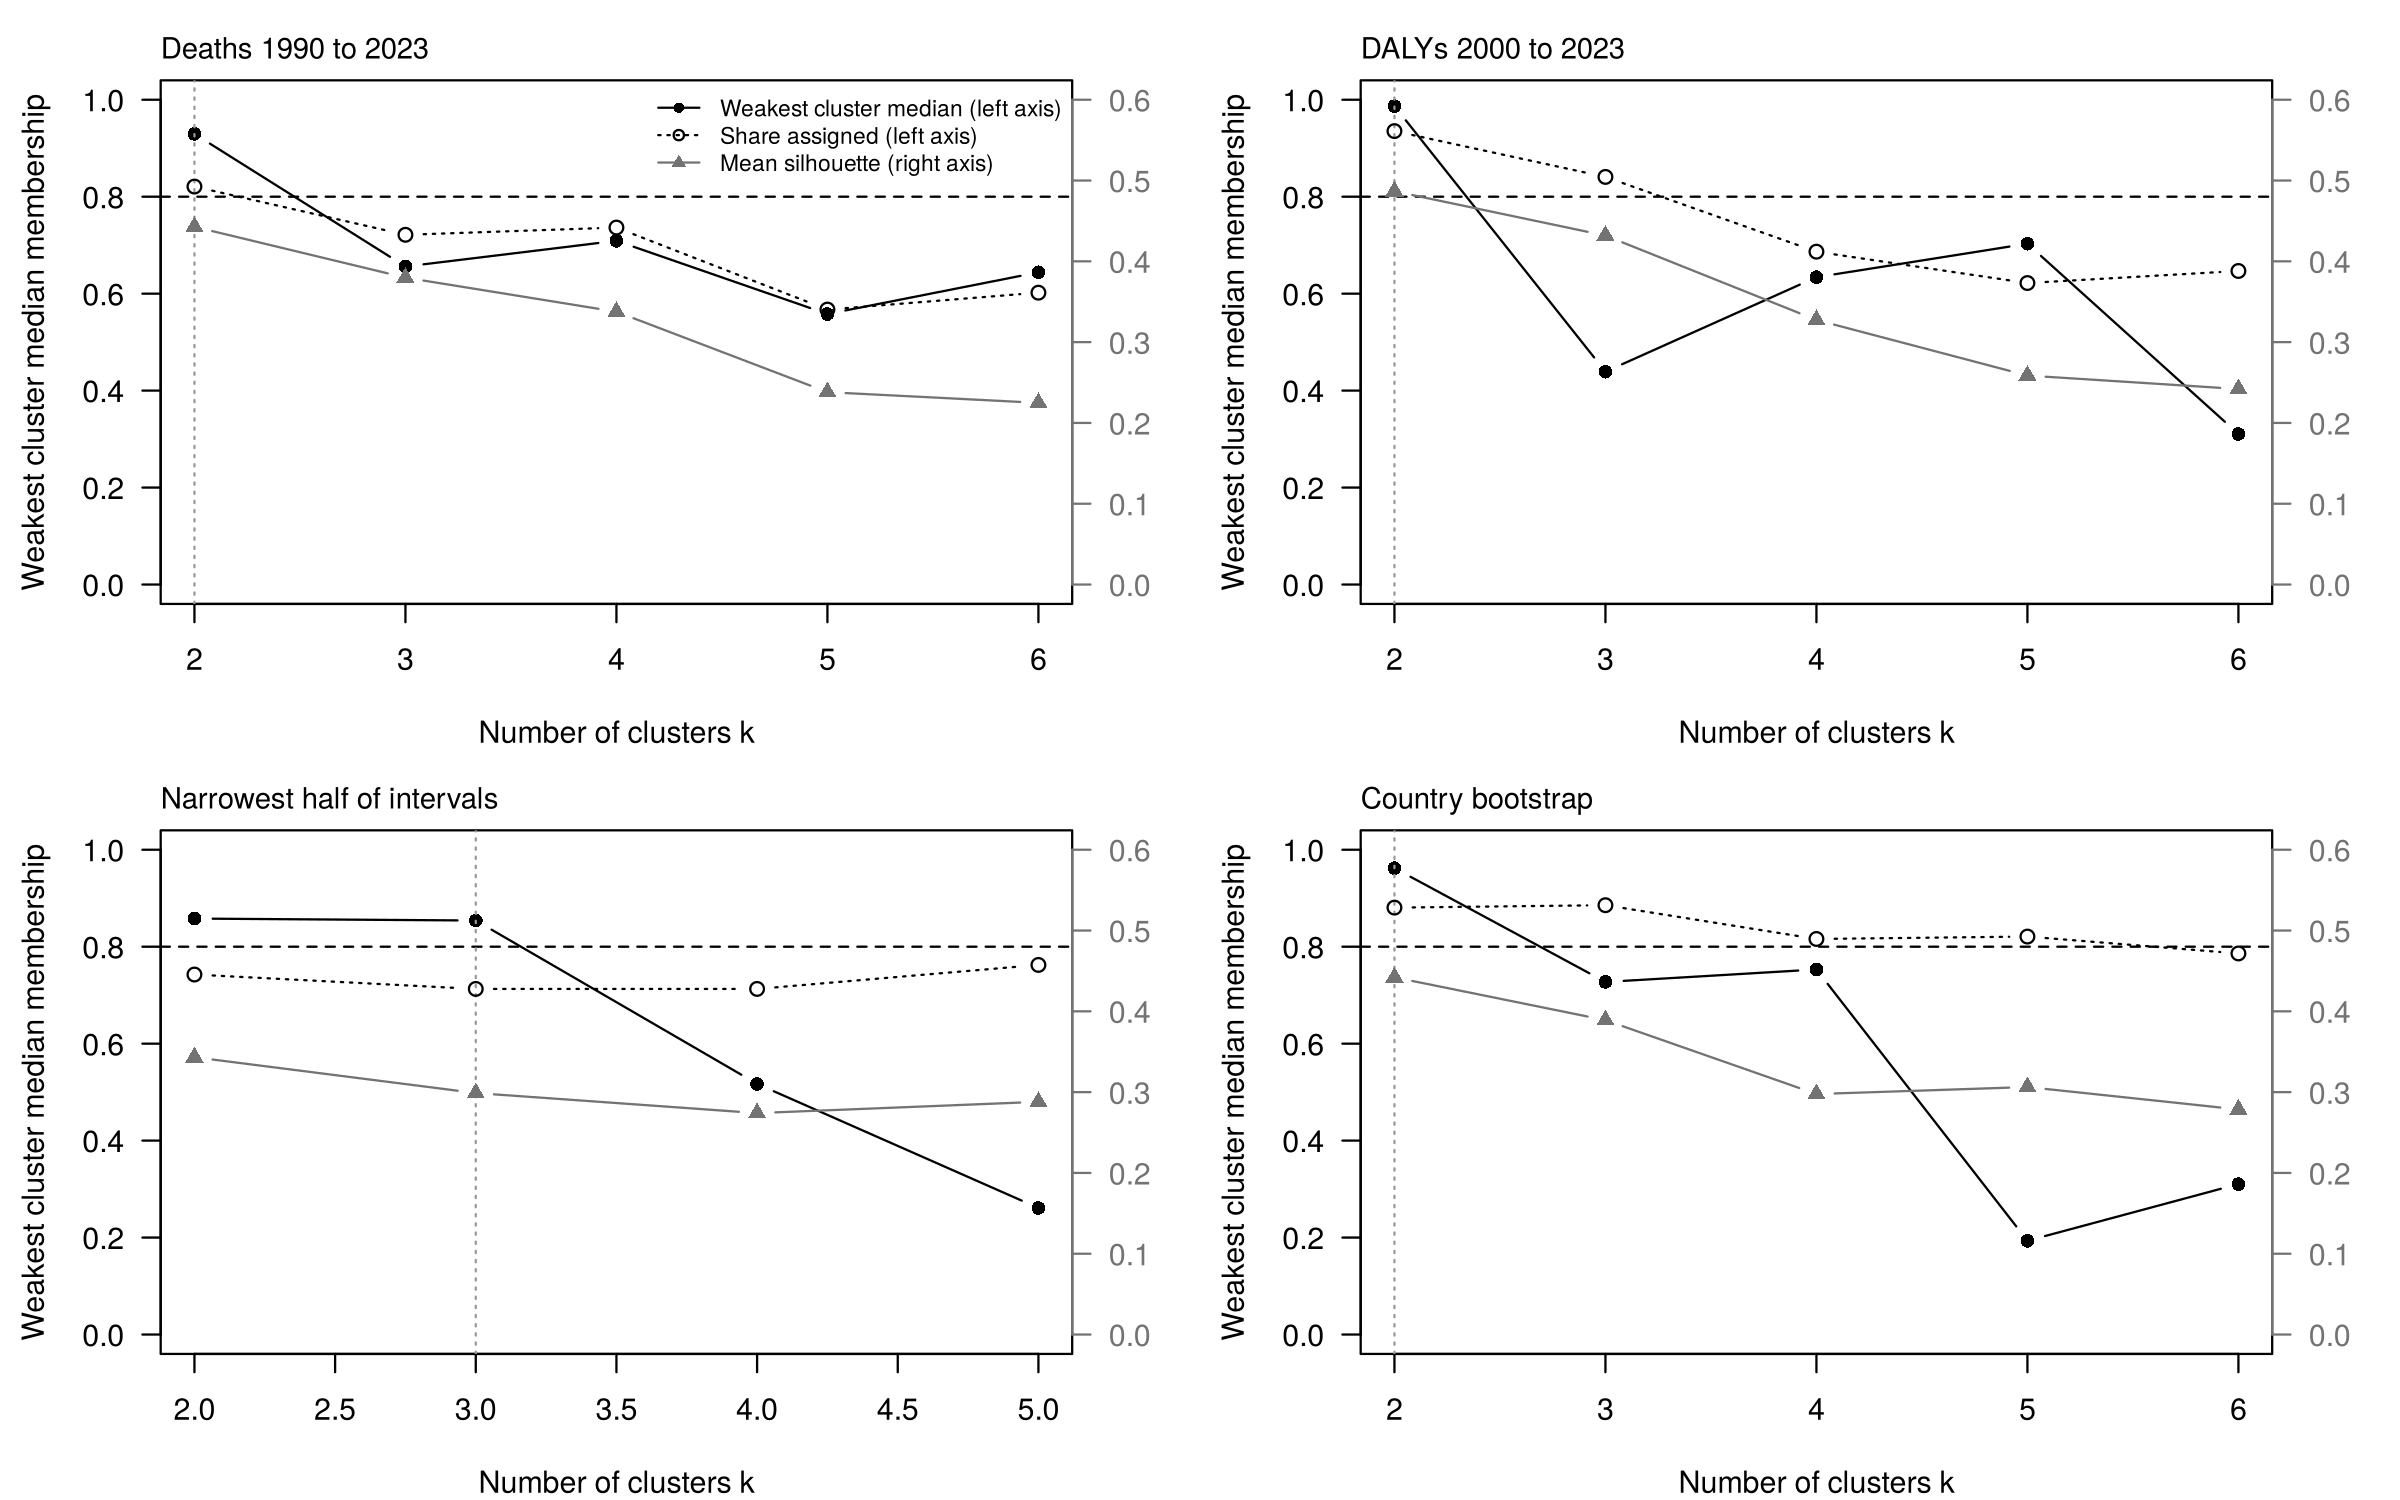
\includegraphics[width=\textwidth]{figS1.png}
\caption{Selection diagnostics for the four robustness runs. Filled circles, weakest cluster median membership probability (left axis); open circles, share of countries assigned (left axis); triangles, mean silhouette width (right axis). Dashed line, the 0.80 rule; dotted vertical, the $k$ the rule selects.}
\label{fig:kall}
\end{figure}


\begin{figure}[h]
\centering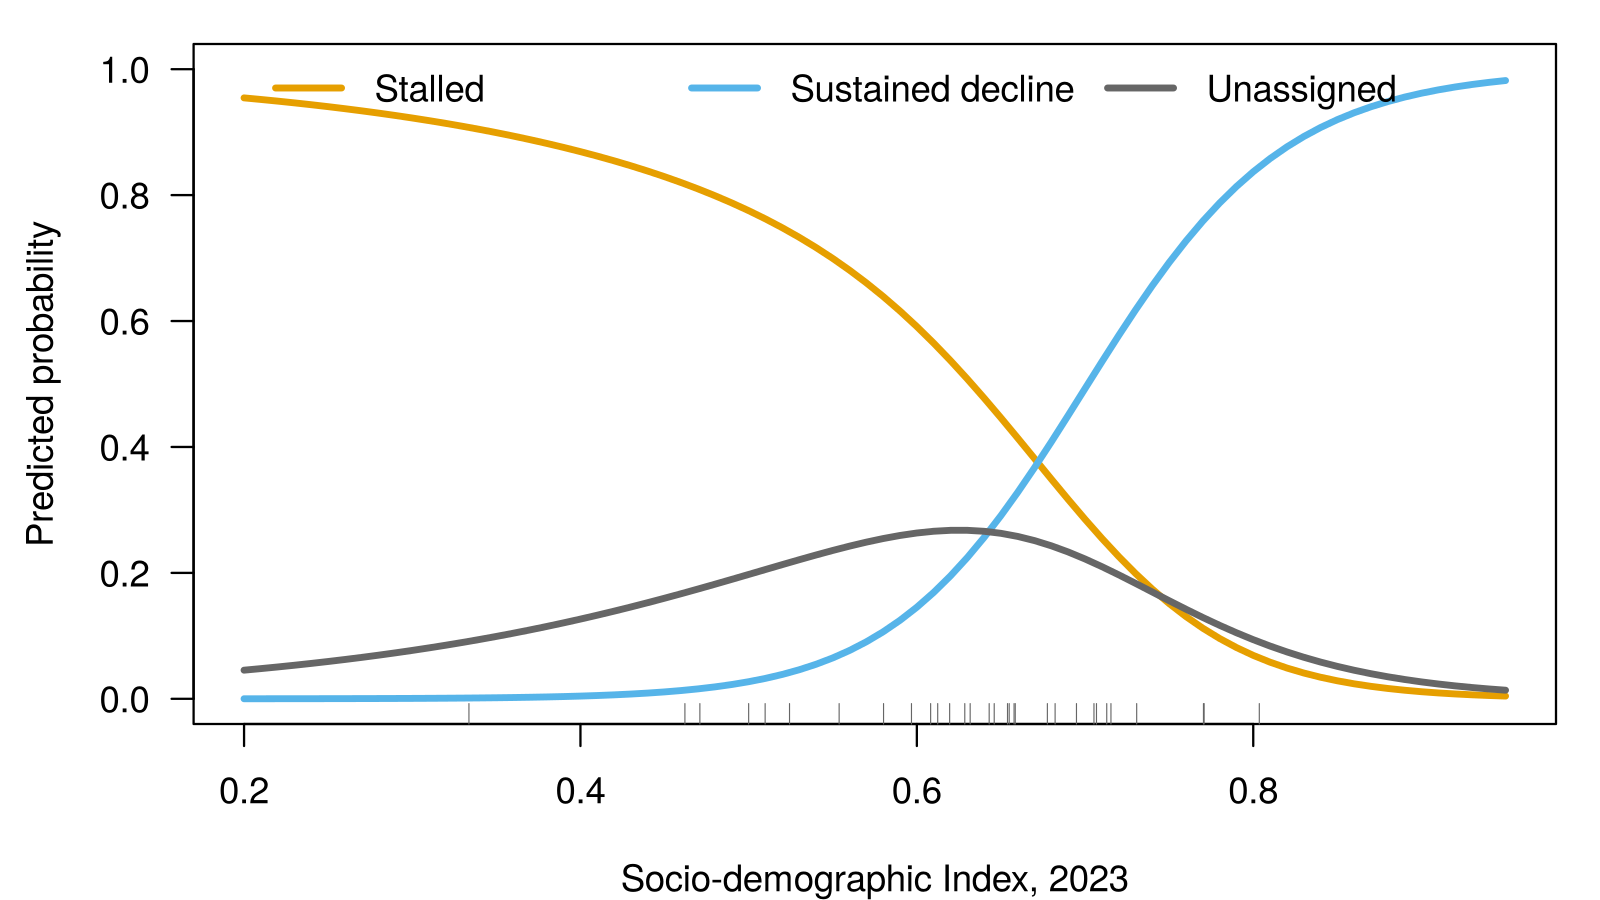
\includegraphics[width=0.7\textwidth]{fig8.png}
\caption{Predicted probability of each membership outcome across the Socio-demographic Index from the multinomial model on SDI alone. Ticks on the horizontal axis mark the SDI of the 31 unassigned countries. Referred to in main-text Section 4.3.}
\label{fig:multinom}
\end{figure}

\clearpage
\section{Reproduction}

The analysis runs in R 4.3.3 with the packages \texttt{cluster}, \texttt{nnet} and \texttt{maps}, all available from CRAN or from Ubuntu's \texttt{r-cran-*} repositories; no other packages are needed. The supplementary archive contains:

\begin{description}
\item[\texttt{data/panel\_cvd.csv}] age-standardised and all-ages cardiovascular DALY rates with intervals, 203 countries by 34 years.
\item[\texttt{data/panel\_cvd\_deaths.csv}] the same for death rates.
\item[\texttt{data/sdi\_2023.csv}, \texttt{superregion.csv}, \texttt{income\_group.csv}] covariate lookups.
\item[\texttt{data/cvd\_case\_study\_membership.csv}] the country list and metadata that fixes the analysis set.
\item[\texttt{analysis/final\_analysis.R}] one run from one seed (20261003) with $B = 1{,}000$ that produces every table and figure in the main text and this supplement; about 75 seconds on a laptop.
\item[\texttt{analysis/build\_supplement\_tables.R}] renders the supplementary tables from the saved workspace.
\item[\texttt{analysis/unwrap.R}, \texttt{unwrap\_csv.R}] helpers that convert connector responses into the panel files, for anyone repeating the extraction.
\end{description}

\noindent The core of the framework, main-text equations (6) to (8), is the following function, reproduced from \texttt{final\_analysis.R}:

\begin{lstlisting}[language=R]
stability <- function(Y, S, hc, k, B, mode = "value") {
  ref <- cutree(hc, k); shape <- sweep(Y, 1, rowMeans(Y))
  agree <- numeric(nrow(Y)); drawn <- numeric(nrow(Y))
  for (b in 1:B) {
    if (mode == "value") {
      Yb  <- Y + matrix(rnorm(length(Y)), nrow(Y)) * S     # equation (6)
      idx <- 1:nrow(Y)
      clb <- cutree(hclust(dist(sweep(Yb, 1, rowMeans(Yb))), "ward.D2"), k)
    } else {                                                # country bootstrap
      idx <- sort(unique(sample(nrow(Y), replace = TRUE)))
      clb <- cutree(hclust(dist(shape[idx, ]), "ward.D2"), k)
    }
    lab <- apply(table(clb, ref[idx]), 1, which.max)       # equation (7)
    agree[idx] <- agree[idx] + (lab[clb] == ref[idx])
    drawn[idx] <- drawn[idx] + 1
  }
  list(ref = ref, p = agree / drawn)                         # equation (8)
}
\end{lstlisting}

\noindent The uncertainty aware choice of $k$ (equation (10)) is then one line: the largest $k$ for which \texttt{min(tapply(p, ref, median)) >= 0.80}.

\end{document}
